\PassOptionsToPackage{unicode}{hyperref}
\documentclass[9pt]{beamer}

\usetheme{TUDo}
\usefonttheme[onlymath]{serif}

\usepackage{fixltx2e}

% Sprachumgebung
\usepackage{polyglossia}
\setmainlanguage{german}

% Mathematik
\usepackage{amsmath}
\usepackage{amssymb}
\usepackage{mathtools}
\usepackage{cancel}

\usepackage[
  math-style=ISO,
  bold-style=ISO,
  sans-style=italic,
  nabla=upright,
  partial=upright,
]{unicode-math}

\usepackage{fontspec}
\setsansfont{TeX Gyre Heros}

%Links
\usepackage{hyperref}
\usepackage{bookmark}

%%%%%%%%%%%%%%%%%%%%%%%%%%%%%%%%%%%%%%%%%%%%%%%%%%%%%%%%%%%%%%%%%%%%%%%%%%%%%%%%
%%%%%-------------Hier Titel/Autor/Grafik/Lehrstuhl eintragen--------------%%%%%
%%%%%%%%%%%%%%%%%%%%%%%%%%%%%%%%%%%%%%%%%%%%%%%%%%%%%%%%%%%%%%%%%%%%%%%%%%%%%%%%

%Titel:
\title{Das neue \LaTeX-Beamer-Theme der TU~Dortmund}
%Autor
\author{Maximilian Nöthe}
%Lehrstuhl/Fakultät
\institute{Names des Lehrstuhls \\  Name der Fakultät}
%Titelgrafik 
\titlegraphic{Bilder/TUDo-Title-Pic-2.jpg}


\begin{document}

\begin{frame}
  \setcounter{framenumber}{0}
  \titlepage
\end{frame}

\begin{frame}
  \frametitle{Wichtige Hinweise}
  Zu diesem Theme
  \begin{itemize}
    \item Die .sty-Files müssen im gleichen Verzeichnis wie die .tex liegen
    \item Ebenso das mitgelieferte TU-Logo
    \item alternativ können die Dateien an einen beliebigen Ort gelegt werden,
    dies erfordert aber, dass dieser Ordner zu den \texttt{TEXINPUTS} hinzugefügt wird.
  \end{itemize}
  Allgemein zu Beamer und Latex:
  \begin{itemize}
    \item Umfangreicher \LaTeX-Kurs von PeP et Al. \\
    \url{http://toolbox.pep-dortmund.de/files/archive/2014/latex.pdf}
    \item Latex-Beamer Dokumetation:\\
    \url{http://texdoc.net/texmf-dist/doc/latex/beamer/doc/beameruserguide.pdf}
  \end{itemize}
\end{frame}

% \begin{frame}
%     \frametitle{Einführung}
%     \tableofcontents[pausesections]
% \end{frame}

% \section{Blindtext}
% \begin{frame}
% 	\frametitle{Hier steht eine lange, zweizeilige Headline
% 		\newline gefolgt von einem Blindtext}
% Dieser Text dient nur zur Veranschaulichung des Textsatzes. Niemand sollte jemals, aus keinem noch so gutem Grund, so viel Text auf eine Folie packen.

% Dies ist ein Blindtext. Dieser Text ist nicht dafür vorgesehen, den Betrachter in die Welt der Dunkelheit zu führen, sondern dafür, einfach etwas Leeres mit etwas Inhaltlosem zu füllen.

% Dies ist ein Blindtext. Dieser Text ist nicht dafür vorgesehen, den Betrachter in die Welt der Dunkelheit zu führen, sondern dafür, einfach etwas Leeres mit etwas Inhaltlosem zu füllen.

% Dies ist ein Blindtext. Dieser Text ist nicht dafür vorgesehen, den Betrachter in die Welt der Dunkelheit zu führen, sondern dafür, einfach etwas Leeres mit etwas Inhaltlosem zu füllen.

% \end{frame}

% \section{Formelsatz}
% \begin{frame}
% 	\frametitle{Formelsatz}
% 	\begin{block}{Mathematischer Formelsatz ist eine Spezialität von \LaTeX}
%     \begin{align*}
%       \nabla \cdot \vec{E} &= \frac{\varrho}{\varepsilon_0} &
%       \nabla \cdot \vec{B} &= 0 \\
%       \nabla \times \vec{E} &= -\partial_t \vec{B} &
%       \nabla \times \vec{B} &= \mu_0 \vec{\jmath} + \mu_0\varepsilon_0 \partial_t \vec{E}
%     \end{align*}
% 	\end{block}
% \end{frame}

% \section{Das Design}
% \subsection{Farben}
% \begin{frame}
%     \frametitle{Eine TU-Farbpalette: Herbstlich (warm)}
%     Farben können über die üblichen \LaTeX-Pakete wie \emph{xcolor} definiert und mit Hilfe der Beamer Befehle gesetzt werden.
%     Siehe hierzu den vorn verlinkten \emph{Beamer-Users-Guide}. Es wird jedoch empfohlen die TU-Farbpalette zu nutzen:
%     \begin{itemize}
%         \item \textcolor{TUgreen}{Dies istTUgreen}
%             \begin{itemize}
%                 \item \textcolor{TUlightgreen}{Dies ist TUlightgreen}
%                 \item \textcolor{TUdarkgreen}{Dies ist TUdarkgreen}
%                 \item \textcolor{TUolive}{Dies ist TUolive}
%             \end{itemize}
%         \item \textcolor{TUyellow}{Dies ist TUyellow}
%         \item \textcolor{TUcitron}{Dies ist TUcitron}
%         \item \textcolor{TUlime}{Dies ist TUlime}
%         \item \textcolor{TUorange}{Dies ist TUorange}
%     \end{itemize}
% \end{frame}

% \subsection{Blöcke}
% \begin{frame}
%   \frametitle{Verschiedene Block-Typen}
%   \begin{block}{block}
%     \begin{itemize}
%       \item Standardblock
%       \item für normalen, strukturierten Text
%     \end{itemize}
%   \end{block}
%   \begin{alertblock}{alertblock}
%     \begin{itemize}
%       \item Block in auffallender Farbe
%       \item zur Hervorhebung
%     \end{itemize}
%   \end{alertblock}
%   \begin{exampleblock}{exampleblock}
%     \begin{itemize}
%       \item Ein anderer Block
%       \item für Beispiele
%     \end{itemize}
%   \end{exampleblock}
% \end{frame}

% \section{Beispiel-Folien}
% \subsection{Zweispaltige Layouts}
% \begin{frame}
%   \frametitle{Zwei Spalten für Text}
%   \begin{columns}[T]
%     \begin{column}{0.49\textwidth}
%       \begin{itemize}[<+->] % Die ganze Liste erscheint der Reihe nach
%         \item Erster  Eintrag
%         \item Zweiter Eintrag
%         \item Dritter Eintrag
%       \end{itemize}
%     \end{column}
%     \begin{column}{0.49\textwidth}
%       \begin{enumerate}
%         \item<1-> Dieser Eintrag erscheint direkt
%         \item<2>  Dieser Eintrag erscheint nur nach dem zweiten Klick
%         \item<1-3> Dieser Punkt erscheint von 1-3
%       \end{enumerate}
%       \begin{itemize}[<+->]
%         \item Erster  Punkt
%         \item Zweiter Punkt
%         \item Dritter Punkt
%       \end{itemize}
%     \end{column}
%   \end{columns}
% \end{frame}

% \begin{frame}
%   \frametitle{Je eine Spalte für Text/Bild}
%   % Für Bilder Argument T benutzen:
%   \begin{columns}[T]
%     \begin{column}{0.49\textwidth}
%       \begin{itemize}%[<+->] Kommentar entfernen falls jeder Punkt einzeln erscheinen soll
%         \item Erster Eintrag
%         \item Zweiter längerer Eintrag\\
%         ausgedehnt auf drei Zeilen\\
%         und manuellem Umbruch
%         \item Dritter Eintrag
%         \item Vierter Eintrag
%         \item Fünfter Eintrag mit etwas mehr Text und automatischem Umbruch
%         \item Sechster Eintrag
%         \item[$\,\blacktriangleright$] Siebter Eintrag, anderes Symbol
%       \end{itemize}
%     \end{column}
%     \begin{column}{0.49\textwidth}
%       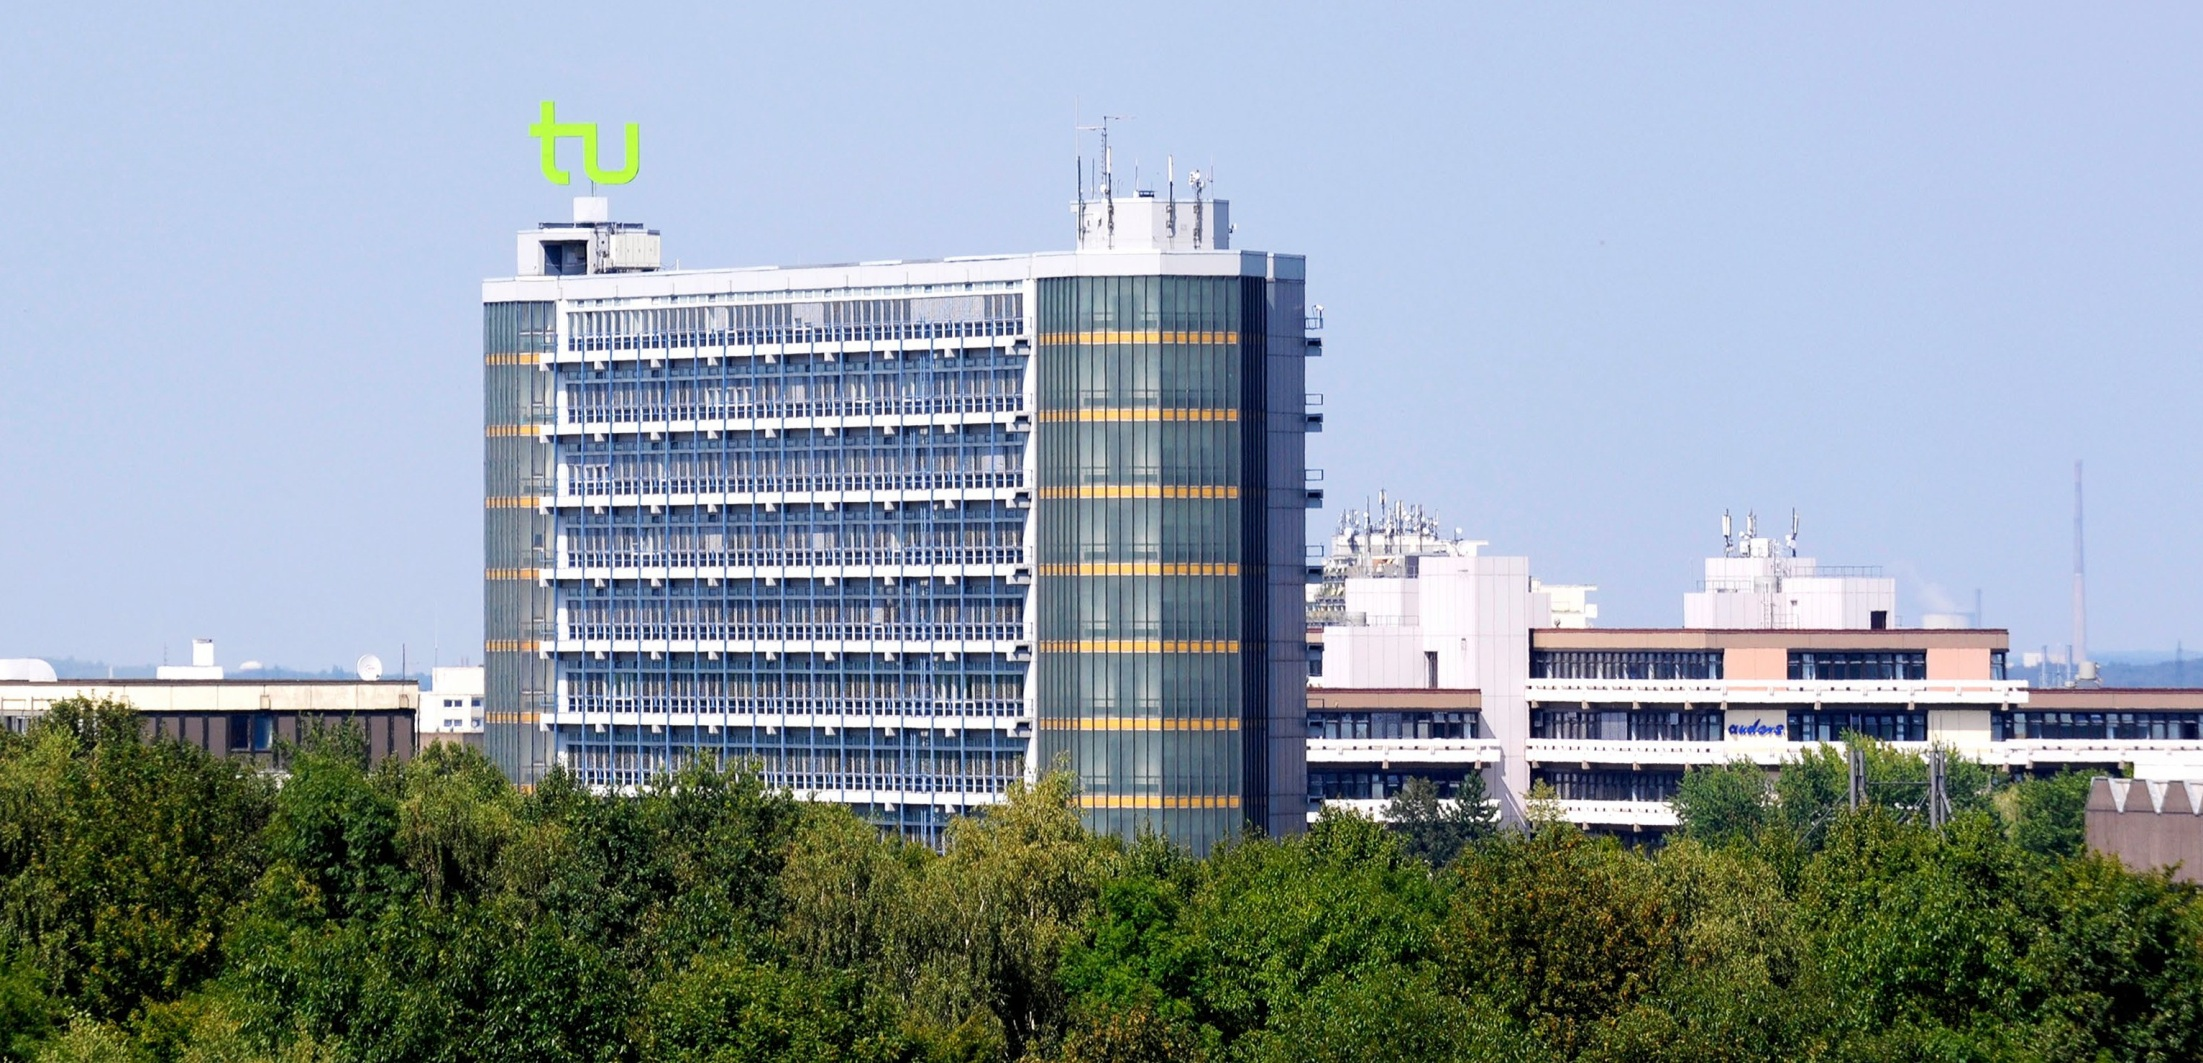
\includegraphics[width=\textwidth]{Bilder/TUDo-Title-Pic-1.jpg}
%       \vspace{5pt}
%       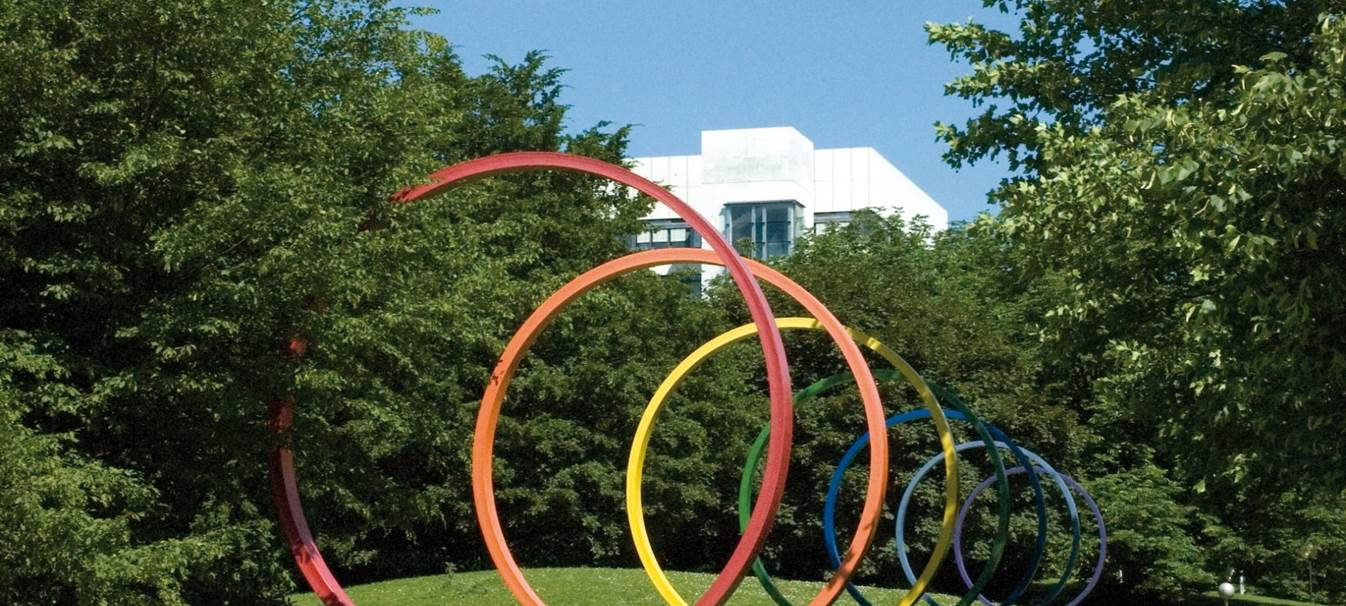
\includegraphics[width=\textwidth]{Bilder/TUDo-Title-Pic-2.jpg}
%     \end{column}
%   \end{columns}
% \end{frame}

% \begin{frame}
%   \frametitle{Zwei Spalten für Text/Bild}
%   % Für Bilder Argument T benutzen:
%   \begin{columns}[T]
%     \begin{column}{0.49\textwidth}
%       \centerline{\textit{\small Feld links oben}}
%     \end{column}
%     \begin{column}{0.49\textwidth}
%       \centerline{\textit{\small Feld rechts oben}}
%       \centerline{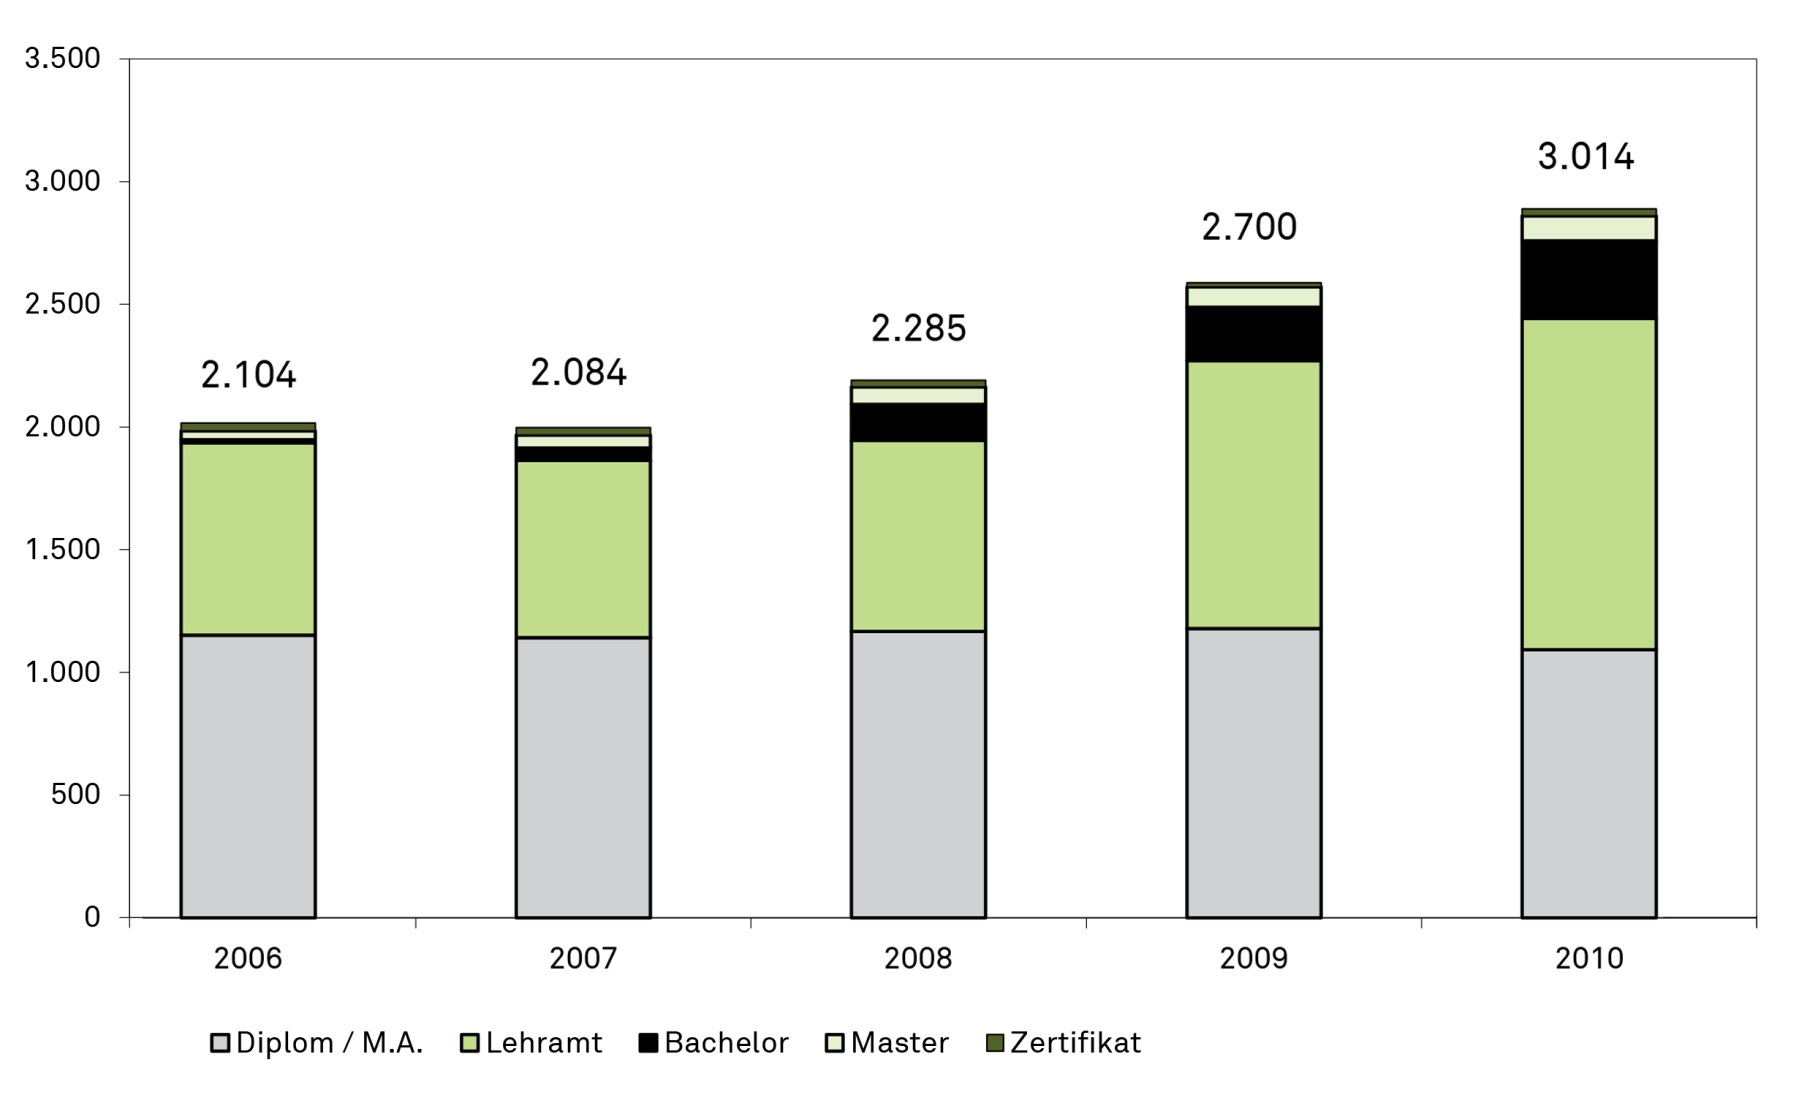
\includegraphics[width=0.75\textwidth]{Bilder/Pic-01.jpg}}
%     \end{column}
%   \end{columns}
%   \medskip
%   \begin{columns}[b]
%     \begin{column}{0.49\textwidth}
%       \centerline{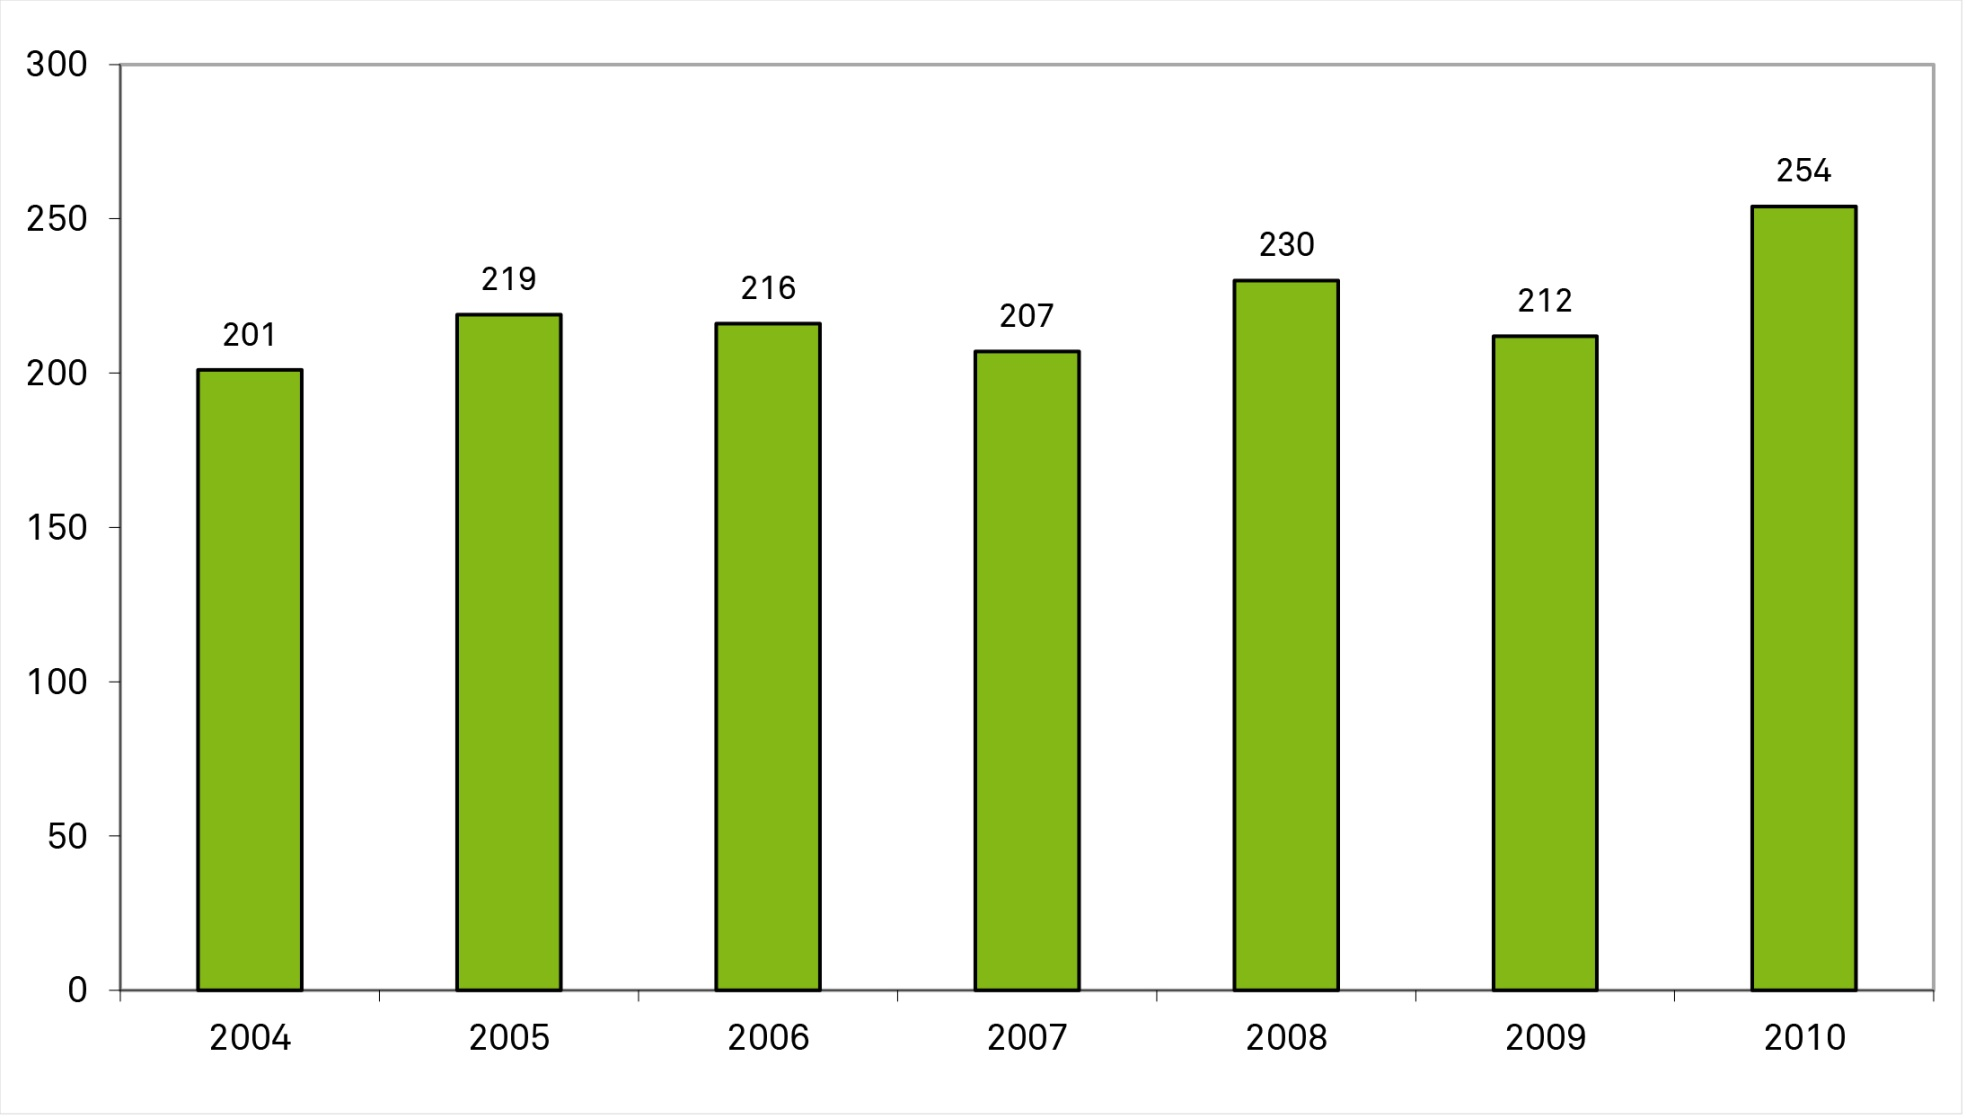
\includegraphics[width=0.75\textwidth]{Bilder/Pic-02.jpg}}
%       \centerline{\textit{\small Feld links unten}}
%     \end{column}
%     \begin{column}{0.49\textwidth}
%       \centerline{\textit{\small Feld rechts unten}}
%     \end{column}
%   \end{columns}
% \end{frame}
\end{document}
